%% Einleitung.tex
\chapter{Introduction}
\label{ch:Introduction}

\section{Motivation}
% Here is the main motivation  - the revolution of earables
With the increasing world population and the growing demand for healthcare, monitoring various biophysiological signals of the body has become increasingly important. 
As a result of increased research and development in this field, several wearable and implantable systems have been developed \cite{loncar-turukaloLiteratureWearableTechnology2019}.
The revolution began with smartphones, followed by other wearables such as watches, and now includes earables.
Earables have emerged as a particularly promising technology for the future of healthcare and lifestyle \cite{trespGoingDigitalSurvey2016, kirkWearablesRevolutionStandardization2014a}. 
The global earable market size was valued in 2022 at around USD 58 million and is expected to rise to 12.6\% until 2030 \cite{GlobalEarphonesHeadphones}.
Most wearables are equipped with various sensors, which are intended to replace a modern medical laboratory through analysis \cite{loncar-turukaloLiteratureWearableTechnology2019}.

% Why earables?
Capturing data using earables has become very popular due to their compact size, their comfortable fit, their easy reachability by hands, and their ability to capture lots of physiological data of the human body \cite{roddigerSensingEarablesSystematic2022a}. 
The fact, that they are very close to the body, especially on a body opening, and can be worn over a long period of time without any issues is a huge advantage compared to other positions to capture such data.
Furthermore, many earables are designed to be discrete, making them a practical option for individuals who want to monitor their health without drawing attention to themselves.
Earables are located near the brain and the major blood vessels on the head and neck and can be worn in or around the ears capturing a variety of biometric data to revolutionize the way we monitor and understand our health such as heart rate, oxygen saturation, and body temperature.

% body temperature
One important aspect of sensing data with earables is the ability to detect changes in body temperature \cite{dolsonWearableSensorTechnology2022, bonziAccuracyPeripheralThermometers2016, NovelWearableDevice2021}. 
Earables equipped with temperature sensors can provide accurate measurements of body temperature throughout the day, which can be used to track patterns and identify potential health issues. 
By monitoring temperature over time, individuals can gain valuable insights into their health and identify potential issues early on.
Knowing a person's exact core body temperature can provide important health insights and information about the person's physiological state.
For example, core body temperature can be an important indicator of fever, as well as infection or inflammation. 
Monitoring this data can provide early insights and enable rapid treatment steps \cite{NovelWearableDevice2021}.
Furthermore, core body temperature can also be used to classify the circadian rhythm of the body \cite{liCircadianRhythmAnalysis2021, juSleepQualityPreclinical2013}.
This controls many physiological processes, revealing possible disturbances when core body temperature is measured continuously.
Athletic performance can also be monitored using core body temperature. Changes in core body temperature can indicate changes in the body's thermoregulatory system that can affect performance and increase the risk of heat illness \cite{gabbettAthleteMonitoringCycle2017, silvaSleepQualityTraining2022}.
%Core body temperature is also closely related to sleep, and monitoring core body temperature can help identify sleep disorders such as sleep apnea \cite{PIIS0022399902, liuSleepSuicideSystematic2020}.
Hormonal changes also affect core body temperature. 
These can, for example, trigger fluctuations in body temperature due to changes in estrogen levels during the menstrual cycle. 
By constantly monitoring body temperature, hormonal changes can be detected and their effects studied \cite{goeckenjanContinuousBodyTemperature2020, charkoudianAutonomicControlBody2017, hamataniEstimatingCoreBody2015}.
In addition, core body temperature monitoring can be useful in diagnosing and treating various medical conditions such as hypothermia, hyperthermia, and sepsis \cite{hardingTemperatureDependenceSleep2019, guilleminaultChronicInsomniaPremenopausal2002, raymannSkinDeepEnhanced2008}.
Overall, continuous core body temperature monitoring can provide valuable insight into a person's health and physiological state and has many potential applications in clinical and research settings.

% Why the ear canal is good for measuring body temperature
The ear canal is a promising location for body temperature measurement because it provides a stable and easily accessible measurement location \cite{ericksonComparisonEarbasedBladder1993}.
In addition, this location is less susceptible to body movement \cite{grossmanFrequencyVelocityRotational1988, kavanaghRoleNeckTrunk2006a}.
In the ear canal, the tympanic membrane is located.
The tympanic is supplied with blood by the branches of the internal carotid artery, which supply blood to the thermoregulation center in the hypothalamus of the brain \cite{moranCoreTemperatureMeasurement2002a}.
Therefore the ear provides high potential in measuring body temperature.

However, the optimal sensor placement and measurement methodology for ear-based temperature monitoring is still an open research question. 
The optimal position for temperature measurement on the ear is quite obvious: the tympanic membrane \cite{childsTympanicMembraneTemperature1999, kimComparisonBilateralEardrum2022, mumaComparisonRectalAxillary1991}.
However, it is not easy to align the infrared sensor with the eardrum. In addition, influencing factors such as ear wax can affect measurement results. 
This raises the question of how measurement results differ at different measurement points on and in the ear. 
By using an alternative measuring point, various influencing factors would be eliminated.
It may also be interesting to see whether the combination of several sensors stabilizes the measurement results.
Another question is how temperature measurements on the ear behave when they are not performed under controlled conditions in the laboratory.
For example, what is the influence of motion artifacts?
With additional sensors, for example, an IMU, it would be possible to detect movements and integrate this knowledge into the erroneous temperature measurement and possibly correct it.

\section{Problem}
Recent research studies have revealed various problems in measuring temperature in the ear.
Discrepancies in temperature-based measurement in the ear have been reported due to factors such as sensor location, skin contact, and calibration \cite{rohrbergTemperatureMeasurementEar1997, gasimAccuracyTympanicTemperature2013, amoateng-adjepongAccuracyInfraredTympanic1999a, hookerScreeningFeverAdult1996a, cattaneoAccuracyPrecisionBody2000}.
The main problem is that the accuracy and reliability of ear temperature measurements can be affected by several factors. 
Measuring temperature at the eardrum is quite complicated to set up since the temperature sensor in the ear canal must be properly aligned. 
Due to the wide variety of ear canal shapes of different individuals, this cannot always be guaranteed.
In addition, influencing factors such as earwax can affect the path to the eardrum and thus also the temperature measurement and all the advantages of measuring the temperature there.
In particular, it is unclear what effect different measurement positions have on measurement accuracy and reliability.
To address these issues, we will test several hypotheses. 
For example, we may hypothesize that combining signals from different sensors will improve measurement accuracy and reliability.
In addition, it is conceivable that other signals like IMU can be used to detect measurement errors, sports activities, or the like.
Various metrics are used to evaluate the accuracy and reliability of ear temperature measurements, such as Mean Squared Deviation and correlation.
Through our studies, we hope to help improve the accuracy and reliability of temperature-based measurements in the ear and thus contribute to medical diagnostics.

\section{Question}
This master's thesis examines temperature sensors, each placed at different locations in and around the ear canal comparing the sensor measurements with those of a medically certified thermometer, considered here as the ground truth.
The research objective is to combine and/or compare different positions for temperature-based measurement in and around the ear and investigate how this affects the accuracy and stability of the measurements.
Additionally, it is interesting to see if other sensor information can be used to filter out potential errors and optimize results. These include, for example, audio signals or an IMU signal. The resulting location or combined locations for the measurement will then be taken as a basis to detect a temperature-dependent event of the body and evaluate if this provides conclusive results.
Various metrics such as Mean Squared Deviation and correlation are used to measure the accuracy and stability of the measurements.
% TODO: maybe more metrics
It is hoped that combining different positions for measurement in the ear will lead to more accurate and stable measurements and that using other sensor information to filter errors may help to further improve the results. It is also expected that the identified optimal location for measurement will be able to detect a temperature-dependent event of the body with high accuracy.

% Wenn du etwas mehr gelesen hast was man konkret mit temperatur machen kann dann können wir mal darüber reden was davon in frage kommt für eine mögliche application. Sollte aber evtl. eher optional sein, je nach aufwand der application (z.b. zyklus tracking zu gefährlich für MA wegen knapper Zeit vs. mind 2 bis 3 Monate tracken für sinnvolle daten)

\section{Planned Approach}
We will use the OpenEarable platform to attach various temperature sensors to the ear canal. 
The sensors will be placed at various locations including the concha, inside the ear canal, one pointing to the eardrum, and behind the pinna.
The exact positions can be explored in figure \ref{fig:ear_measurement_positions}.
Participants will be asked to wear the sensors on one ear in a study under laboratory conditions.
The resulting data will be collected and analyzed afterward to determine the best sensor position for ear-based temperature measurement. 
This position will then be used to classify temperature-related events of the body.

To gain additional insight, we also plan to take temperature measurements during different activities to see how the measurements behave in different situations. We will select relevant activities and compare them to results from the literature to see if our results are consistent with those from previous studies.

\begin{figure}
    \centering
    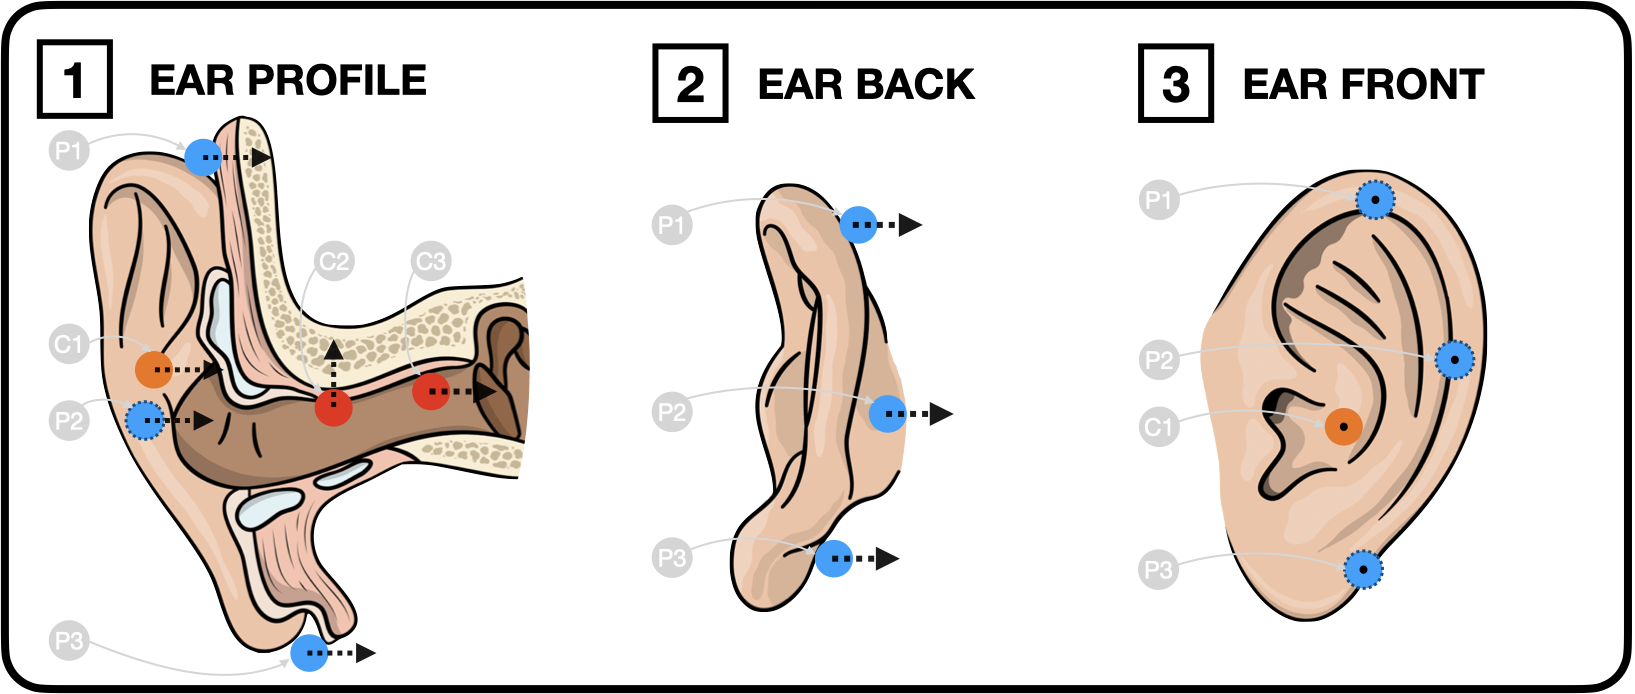
\includegraphics[scale=0.26]{thesis-doc/images/ear_measurement_points/emp.png}
    \caption{TODO} %TODO: make caption
    \label{fig:ear_measurement_positions}
\end{figure}

\section{Expected Results}
We expect that our study will provide insights into the placement of sensors for temperature monitoring in or directly on the ear.
For this purpose, it is possible that this will be done by one sensor or by a combination of several sensors.
Possible variations in temperature measurements at different positions in the ear canal will be identified in order to be able to adequately predict the temperature at the ear in everyday situations.
Our results will support the development of more accurate and reliable wearable devices for biometric applications. 
In addition, the optimally determined position will serve as a new basis for the analysis of various body temperature-changing events.